\clearpage
\section{Paisaje} \label{sec:paisaje}

En esta práctica vamos a centrarnos en el uso del \gls{CSS} y de las animaciones. Antes de nada, haremos una pequeña introducción a qué es y como funciona \gls{CSS} y como podemos trabajar con el en Ionic2.

\gls{CSS} es un leguaje utilizado para definir la presentación de un documento estructurado escrito en un lenguaje de marcado. Esto, cuando trabajamos con tecnología Web, se refiere al estilo a aplicar nuestra página, la cual está escrita en \gls{HTML}, que actúa como lenguaje de marcado. Así, mientras que nuestro código \gls{HTML} contiene la información, el código \gls{CSS} define la presentación. Con esta separación entre información y presentación se consigue un mayor control y modularidad.

La última especificación de \gls{CSS} es la número 3, la que se conoce como \gls{CSS3}.

Una de las características mas útiles y que más han evolucionado son las animaciones. Muy útiles a la hora de realizar páginas más vistosas. Con ellas, podemos definir transiciones entre estilos definidos en el \gls{CSS}. Estas animaciones constan de dos elementos:

\begin{enumerate}
  \item Uno que describe la animación que se produce en la transición.
  \item Otro que define los frames del estado inicial y final de la animación. Incluso se puede llegar a definir estados intermedios.
\end{enumerate}

Para facilitar el trabajo con \gls{CSS}, Ionic2 incluye \gls{Sass}. \gls{Sass} es un lenguaje que amplia las capacidades de \gls{CSS}. Los navegadores no entienden el lenguaje \gls{Sass}, por lo que es necesario traducirlo a \gls{CSS}, de forma similar a lo que ocurre con TypeScript y JavaScript.

\gls{Sass} utiliza dos tipos de sintaxis, siendo validas cualquiera de las dos:
\begin{enumerate}
  \item La sintaxis original, en la que se utiliza la identación para separar los distintos bloques. La extensión de los ficheros escritos con esta sintaxis es .Sass.
  \item Una sintaxis más parecida a la usada en \gls{CSS}, con el uso de las llaves ({}) para separar los bloques y del punto y coma (;) al final de cada línea. En este caso la extensión de los ficheros es .scss.
\end{enumerate}

\tipbox{Si nos fijamos al crear un nuevo proyecto o una nueva página, las hojas de estilo que aparecen son nombradas como *.scss y no como *.css.
Ionic, a la hora de compilar la aplicación, es lo suficientemente autónomo como para utilizar este fichero y los estilos en él definido en el ámbito de nuestro componente, sin necesidad de indicarlo manualmente.}

Alguna de las capacidades que incluye \gls{Sass} y que encontraremos de gran utilidad son:
\begin{enumerate}
  \item La posibilidad de definir variables.
  \item El uso de mixins\footnote{\url{http://sass-lang.com/guide#topic-6}}, gracias a los cuales nos evitaremos el tener que duplicar código.
  \item Anidar los estilos en bloques.
  \item Poder hacer uso de directivas de control y expresiones como \emph{if, for, each, ...}.
  \item Herencias de etilos como ocurre en lenguajes orientados a objetos.
  \item \ldots{}
\end{enumerate}

Para más información sobre \gls{Sass}, podemos visitar su página de documentación \url{http://Sass-lang.com/documentation/file.Sass_REFERENCE.html}.

Por último, y antes de entrar en faena, debemos mencionar el control de animaciones que nos ofrece Angular (que recordemos, es la base sobre la que funciona Ionic2). Las animaciones en Angular funcionan de la misma forma que las animaciones \gls{CSS}, facilitándonos el uso de estas en determinados escernarios. Las animaciones de Angular se definen como parte de los metadatos del \emph{@component} en los que se van a usar. En la definición de una animación se definen tres elementos principales que aunque veremos con más profundidad más adelante, durante el desarrollos, vamos a enumerar a continuación:

\begin{enumerate}
  \item El \emph{Animation trigger} o \emph{trigger} a secas. Es el disparador que se vincula al elemento \gls{HTML}. Dentro de él se define toda la animación. Un componente puede tener asignado cualquier cantidad de \emph{trigger}.
  \item Los \emph{states}, o estados, son aquellos en los cuales puede estar el \emph{trigger} y que definen el estilo que se tiene que aplicar al elemento cuando se encuentra en ese estado.
  \item Y las \emph{transitions} o transiciones las cuales definen la animación que se produce cuando hay un cambio de estados.
\end{enumerate}

Para poder ver en acción las animaciones, vamos a crear un paisaje con elementos animados. El resultado será algo como lo siguiente:

\begin{figure}[H]
\centering
    \centering
        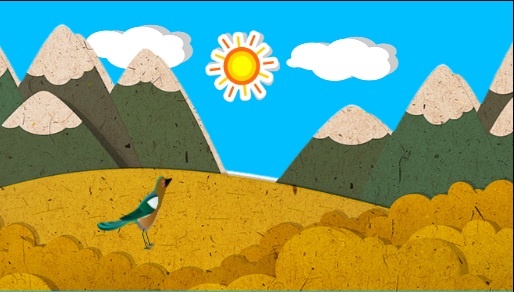
\includegraphics[width=0.8\textwidth]{Figures/ch2/Landscape/final_day}
        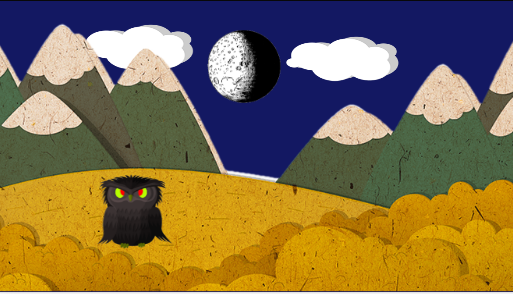
\includegraphics[width=0.8\textwidth]{Figures/ch2/Landscape/final_nigth}
    \caption{Nuestra aplicación nos mostrará un paisaje, en el que podremos cambiar entre noche y día.}
\end{figure}

\subsection{Primeros pasos. El cielo.}


Empezaremos como siempre, creando un nuevo proyecto dentro de nuestro directorio de trabajando utilizando el Ionic CLI. En mi caso, he decidido llamarle Landscape:

\begin{lstlisting}[language=bash]
  # ionic start Landscape blank --v2
\end{lstlisting}

Empezaremos editando los ficheros \emph{home.html} y \emph{home.scss} (podemos renombrar la página con un nombre más descriptivo si queremos, lo cual sería recomendable en caso de tener más páginas, pero en este caso, no será necesario). Eliminaremos todo el contenido de del fichero HTML y añadiremos un \emph{div} que actuara como ``lienzo'' para nuestro paisaje. A este elemento le vamos a asignar las clases \emph{canvas} y \emph{sky}, haciéndolo más reconocible.

\begin{lstlisting}[style=htmlcssjs,frame=tlrb, xleftmargin={0.2cm}]
  <div class="canvas sky" ></div>
\end{lstlisting}

En cuanto al fichero \emph{.scss}, añadiremos los estilos para nuestro nuevo elemento. Estos estilos los anidaremos dentro del elemento \emph{page-home}. El elemento \emph{page-home} es el que representa a nuestro componente (la opción \emph{selector} del metadata de un \emph{@component} es la que indica el nombre de este selector).

\begin{lstlisting}[style=htmlcssjs,frame=tlrb, xleftmargin={0.2cm}]
  page-home {
    .canvas.sky{
      height: 100%;
      width: 100%;
      background-color: #00BFFF;
    }
  }
\end{lstlisting}

Aquí vemos una de las capacidades comentadas de \emph{Sass}. Hemos anidado los estilos que aplican a las clases \emph{.canvas.sky} dentro de \emph{page-home}. Para ver la diferencia con \emph{CSS}, podemos ver el código que esto genera al ser compilado:

\begin{lstlisting}[style=htmlcssjs,frame=tlrb, xleftmargin={0.2cm}]
  page-home .canvas.sky {
    height: 100%;
    width: 100%;
    background-color: #00BFFF;
  }
\end{lstlisting}

Resulta más intuitivo definir los estilos anidando las reglas de igual forma que está definidos los elementos dentro del \gls{DOM} de la página, que la forma que se utiliza en \gls{CSS}, en la que la relación padre e hijos se representa separando los identificadores con un espacio.

Si ejecutamos en estos momentos la aplicación, no veremos más que una pantalla azul, la cual hará la función de cielo en nuestro paisaje. Será sobre este cielo donde iremos añadiendo elementos.

\subsection{Animaciones definidas sobre el componente. El sol y la luna.}


Empezaremos por incluir un sol, y al igual que hicimos con el canvas, este será representado por un componente \gls{HTML} al que le añadiremos como fondo la imagen de un sol. Esta imagen tendremos que ponerla dentro de la carpeta \emph{/src/assets} para que, una vez se genere la aplicación, esta sea incluida. Yo he creado una carpeta intermedia llamada \emph{landscape} para tener las imágenes mas ordenadas. Así pues, añadimos el sol dentro de nuestro ``lienzo'' y lo estilamos dentro de nuestro fichero \emph{scss}:

\noindent
\begin{minipage}[t]{.48\textwidth}
{\begin{lstlisting}[title={home.html}, style=htmlcssjs,frame=tlrb,xleftmargin={0.2cm}]
<div class="canvas sky" >
  <div class="celestial sun" ></div>
</div>
\end{lstlisting}}
\end{minipage}\hfill
\noindent
\begin{minipage}[t]{.48\textwidth}
{\begin{lstlisting}[title={home.scss}, style=htmlcssjs,frame=tlrb,xleftmargin={0.2cm}]
page-home {
 .canvas.sky{ ... }
 .celestial{
     position: fixed;
     height: 100px;
     width: 100px;
     left: 40%;
     top: 10%;
     background-size: contain;
     background-repeat: no-repeat;
     &.sun{
       background-image: url(../assets/landscape/sun.png);
     }
   }
}
\end{lstlisting}}
\end{minipage}

Si nos fijamos, he asignado dos clases al elemento que contendrá mi sol, la clase \emph{celestial} y la clase \emph{sun}. A estas clases las he dado estilo anidando la clase \emph{sun} dentro de la clase \emph{celestial}, pero con un elemento diferente a la de otras anidaciones. En el caso de la clase \emph{sun}, le he antepuesto el carácter \emph{\&}. ¿Y qué significa esto?. A la hora de generar el fichero \emph{CSS}, el compilador sustituirá este carácter por el selector del estilo padre, es decir, por \emph{.celestial}. Para que nos hagamos una mejor idea:

\begin{tikzpicture}[>=stealth, thick]

\node (A) at (-4,0) [draw, process, text width=5cm, minimum height=0.5cm, align=flush center]
{
.celestial \{
  .sun \{ ... \}
\}
};

\node (B) at (4, 0) [draw, process, minimum height=0.5cm, align=flush center]
{
.celestial .sun \{ ... \}
};

\node (C) at (-4, -1) [draw, process, text width=5cm, minimum height=0.5cm, align=flush center]
{
.celestial \{
  \&.sun \{ ... \}
\}
};

\node (D) at (4, -1) [draw, process, minimum height=0.5cm, align=flush center]
{
.celestial.sun \{ ... \}
};

\draw[->] (A) -- node[above]{Compila a} (B);
\draw[->] (C) -- node[above]{Compila a} (D);
\end{tikzpicture}

Con esto conseguimos tener nuestro sol en medio del cielo azul, pero uno de los comportamientos que buscamos es que nuestro paisaje tenga una versión nocturna  además de una diurna. Para hacer esto, vamos a definir un estado dentro de nuestro \emph{@component} que defina si es de día, o de noche, y haremos que este estado cambie al pulsar sobre nuestro sol. Para esto solo será necesario vincular el evento de \emph{click} sobre el sol a una función que haga cambiar la variable de estado de nuestro componente:

\noindent
\begin{minipage}[t]{.48\textwidth}
{\begin{lstlisting}[style=htmlcssjs,frame=tlrb, xleftmargin={0.2cm}]
<div class="canvas sky" >
  <div class="celestial sun" (click)="toogleState()" ></div>
</div>
\end{lstlisting}}
\end{minipage}\hfill
\noindent
\begin{minipage}[t]{.48\textwidth}
{\begin{lstlisting}[style=htmlcssjs,frame=tlrb, xleftmargin={0.2cm}]
export class HomePage {
  state: string = 'day';

  // otras funciones

  toogleState() {
    this.state = 'day' == this.state ? 'night' : 'day';
  }
}
\end{lstlisting}}
\end{minipage}

Ya tenemos una variable que almacena el estado y que podemos cambiar pulsando nuestro sol, pero no vemos como esto se refleja en nuestro paisaje (a no ser que depuremos la aplicación o hagamos que imprima el valor por consola). Vamos por fín a hacer uso de las animaciones. La primera va a ser muy sencillita, cambiar el color del cielo a uno mas nocturno. En primer lugar vamos a crear una animación de Angular que haga esto y la añadiremos a nuestro componente. Para hacer esto modificamos el metadata de nuestro componente de la siguiente manera:

{\begin{lstlisting}[style=htmlcssjs,frame=tlrb, xleftmargin={0.2cm}]
@Component({
  selector: 'page-home',
  templateUrl: 'home.html',
  animations: [
    trigger('skyState', [
      state('day', style({
        backgroundColor: '#00BFFF'
      })),
      state('night',   style({
        backgroundColor: '#131862'
      })),
      transition('day <=> night', animate('1s')),
    ]),
  ]
})
\end{lstlisting}}

No nos olvidemos de importar las nuevas clases que vamos a utilizar: https://angular.io/docs/ts/latest/api/core/index/trigger-function.html

{\begin{lstlisting}[style=htmlcssjs,frame=tlrb, xleftmargin={0.2cm}]
import { Component, ElementRef, ViewChild, AfterViewInit, trigger, state, style, transition, animate} from '@angular/core';
\end{lstlisting}}

Veamos que es lo hemos definido:

\begin{enumerate}
  \item Hemos definido el metadato \emph{animations} de nuestro componente como una lista en la que de momento solo definiremos un \emph{trigger}\footnote{\url{https://angular.io/docs/ts/latest/api/core/index/trigger-function.html}}.
  \item Este \emph{trigger}, que es una llamada al constructor de la clase \emph{trigger}, lo hemos nombrado \emph{skyState} (primer parámetro que acepta el constructor).
  \item Como segundo parámetro le pasamos una lista de estados y transiciones que definen las animaciones.
  \item Hemos definido dos estados mediante la clase \emph{state}\footnote{\url{https://angular.io/docs/ts/latest/api/core/index/state-function.html}}:
  \begin{enumerate}
    \item Un estado llamado \emph{day}, con un estilo que define el color de fondo de la misma manera que se definen las reglas en \gls{CSS}.
    \item Un estado llamado \emph{night}, que también define también el color de fondo, pero cambiando el valor de este.
  \end{enumerate}
  \item Junto a los estados hemos definido una transición. Como primer parámetro, le pasamos el nombre de los estados definidos previamente entre los que se hace el cambio, y la dirección entre ellos en las que se da (la flecha <=> indica bidireccionalidad, mientras que una flecha tipo =>, indicaría solo un sentido). Como segundo parámetro, seleccionamos el tipo de animación que queremos mediante una clase \emph{animate}\footnote{\url{https://angular.io/docs/ts/latest/api/core/index/animate-function.html}}, en este caso, queremos que la animación dure un segundo en completarse ('1s').
\end{enumerate}

Por último nos quedaría vincular nuestro \emph{trigger} a nuestro cielo y al estado definido dentro del componente. Esto se hace directamente editando el elemento \gls{HTML}.

{\begin{lstlisting}[style=htmlcssjs,frame=tlrb, xleftmargin={0.2cm}]
<div class="canvas sky" [@skyState]="state" >
\end{lstlisting}}

Que el sol aparezca en medio de un cielo nocturno no es muy común, necesitaremos hacer uso de otra animación para solucionar esto. En esta ocasion en vez de contar con un único elemento al que le cambiamos el estilo, añadiremos uno nuevo que representará la luna. Este elemento tendrá varios estilos en común con el sol definido anteriormente, por lo que compartirán clase \emph{celestial} (ahora le vemos el sentido a la separación de estilos que hicimos anteriormente entre \emph{celestial} y \emph{sun}). El ver aparecer o desaparecer estos cuerpos celestiales en centro de la pantalla no es lo más bonito, así que para esta animación haremos que el cuerpo celeste aparezca por el borde superior, y desaparezca por el borde inferior según le toque. Nos vamos a ayudar de la regla \emph{top} que define \gls{CSS}, con la cuál podemos definir a que distancia respecto al borde superior se posiciona el elemento en cuestión (de igual manera, la regla \emph{left} define la distancia respecto al borde izquierdo). Entre los valores que acepta, se puede indicar un tanto por ciento respecto a la altura del elemento padre y así, jugando con este valor, podremos crear la animación que queremos. Empezamos definiendo nuestro nuevo elemento y las posiciones de origen.

\noindent
\begin{minipage}[t]{.48\textwidth}
{\begin{lstlisting}[style=htmlcssjs,frame=tlrb, xleftmargin={0.2cm}]
<div class="canvas sky" [@skyState]="state" >
  <div #sun class="celestial sun" (click)="toogleState()" ></div>
  <div #moon class="celestial moon" (click)="toogleState()" ></div>
</div>
\end{lstlisting}}
\end{minipage}\hfill
\noindent
\begin{minipage}[t]{.48\textwidth}
{\begin{lstlisting}[style=htmlcssjs,frame=tlrb, xleftmargin={0.2cm}]
.celestial{
  position: fixed;
  height: 100px;
  width: 100px;
  left: 40%;
  top: 10%;
  background-size: contain;
  background-repeat: no-repeat;
  &.sun{
    background-image: url(../assets/landscape/sun.png);
  }
  &.moon{
    background-image: url(../assets/landscape/moon.png);
  }
}
\end{lstlisting}}
\end{minipage}

Crearemos una animación que será la que usen ambos elementos, ambos cuerpos celestiales. En esta animación usaremos dos estados, pero no definiremos ninguno ¿Cómo es esto posible?. Angular ya define dos estados especiales, a saber:

\begin{enumerate}
  \item El estado \emph{void}, que se define un el estado de los elementos que desaparecen.
  \item El estado \emph{*}, es un estado comodín para cuando no existe estado definido.
\end{enumerate}

Con esto presente, crearemos una animación para los siguientes cambios de estado:

\begin{enumerate}
  \item void => *: Esta transición definirá la entrada.
  \item * => *: Por el contrario, esta definirá la salida.
\end{enumerate}

{\begin{lstlisting}[style=htmlcssjs,frame=tlrb, xleftmargin={0.2cm}]
animations: [
  trigger('skyState', [ ... ]),
  trigger('flyInOut', [
    transition('void => *', [
      style({top: '-100%'}),
      animate('1s')
    ]),
    transition('* => void', [
      animate('1s', style({top: '100%'}))
    ])
  ]),
]
\end{lstlisting}}

\notebox{El uso de animaciones de entrada y salida es frecuente, por ello en Angular se han asignado alias especiales a estos cambios de estado. En las transiciones, podemos cambiar la definición de cambio de estado \textbf{'void => *'} por \textbf{':enter'} y \textbf{'* => void'} por \textbf{':leave'}.}

En la transición de entrada, al definir un estilo dentro de la transición, hacemos que antes de que se inicie esta, se le aplique el estilo definido. Así conseguimos que nuestro elemento se coloque por encima de la pantalla. Por el contrario, en la transición de salida, el estilo está definido dentro de la animación. Indicamos así el estilo al finalizar la animación. Este estilo no se guarda, si no que al terminar la animación, el estilo es borrado del elemento.

Solo nos queda asignar la animación a nuestros elementos, pero en esta ocasión no hay estados propiamente dichos, si no que hay que hacer que el elemento aparezca y desaparezca, ¿Cómo hacemos esto?. Usaremos la directriz de Angular \textbf{ngIf}. Esta directriz hace que aparezca o no el elemento asignado en escena según si el valor asignado es \emph{true} o \emph{false}. Usando esta directriz, y la propiedad \emph{state} definida en el componente, nos será fácil conseguir nuestro objetivo:

{\begin{lstlisting}[style=htmlcssjs,frame=tlrb, xleftmargin={0.2cm}]
<div class="canvas sky" [@skyState]="state" >
  <div class="celestial sun" [@flyInOut] *ngIf="state === 'day'" (click)="toogleState()" ></div>
  <div class="celestial moon" [@flyInOut] *ngIf="state === 'night'" (click)="toogleState()" ></div>
</div>
\end{lstlisting}}

\subsection{Animación mediante código JavaScript/TypeScript. El terreno.}


Ya va cogiendo forma nuestro paisaje. Lo siguiente que vamos a añadir va a ser el terreno. Para que nuestro terreno sea un poco más interactivo, vamos a hacer que podamos moverlo con el dedo tanto a la izquierda, como a la derecha. Esto no podemos hacerlo usando las animaciones, ya que el desplazamiento del dedo no es siempre el mismo y las animaciones necesitan tener definido un inicio y un fin. Por tanto, debemos de tratar este movimiento desde el código JavaScript (o TypeScript como en nuestro caso). El gesto de mover un dedo sobre un elemento de nuestra página provoca que se genere un evento JavaScript, que como otro cualquiera, podemos capturar en nuestro código. Este evento nos da información sobre el recorrido que ha hecho nuestro dedo sobre la pantalla, y usando esta información, podremos variar en consecuencia la posición del elemento que representa el terreno.

Vamos a empezar como es normal añadiendo el elemento a nuestro código \gls{HTML} y dándole el estilo deseado.

\noindent
\begin{minipage}[t]{.48\textwidth}
{\begin{lstlisting}[style=htmlcssjs,frame=tlrb, xleftmargin={0.2cm}]
<div class="canvas sky" [@skyState]="state" >
  <div class="celestial sun" [@flyInOut] *ngIf="state === 'day'" (click)="toogleState()" ></div>
  <div class="celestial moon" [@flyInOut] *ngIf="state === 'night'" (click)="toogleState()" ></div>
  <div #landscape class="landscape" ></div>
</div>
\end{lstlisting}}
\end{minipage}\hfill
\noindent
\begin{minipage}[t]{.48\textwidth}
{\begin{lstlisting}[style=htmlcssjs,frame=tlrb, xleftmargin={0.2cm}]
page-home { ... }
  .celestial{ ... }
  .landscape {
    position: fixed;
    height: 100vh;
    width: calc(100vh*1024/373); // El tamano de la imagen es 1024*373, asi que calculamos la relacion alto entre ancho
    background-image: url(../assets/landscape/landscape.png);
    background-size: auto 100%;
    background-repeat: no-repeat;
    pointer-events: none;
  }
}
\end{lstlisting}}
\end{minipage}

Ya que el \emph{div} que contiene la imagen cubre nuestro \emph{sol/luna}, aunque sea con zona transparente, interfiere en el evento del click, evitando que llegue a nuestro cuerpo celeste. Para solucionarlo, añadimos la regla \emph{pointer-events: none;} y controlaremos el evento de pulsación con el dedo desde el  \emph{div} del elemento \emph{canvas}.

Si nos fijamos, en nuestro nuevo \emph{div} aparece un atributo que no habíamos usado anteriormente, \emph{\#landscape}. Al añadir un atributo prefijadocon el caracter almohadilla (\#), le estamos asignando un identificador gracias al cual podremos hacer uso de este elemento desde dentro del \emph{component} y poder ``jugar'' con él. Ya que el tamaño de nuestro terreno se ajusta según la altura de la pantalla, necesitaremos calcular de manera programática el máximo desplazamiento horizontal para evitar que el terreno desaparezca por uno de los bordes laterales. Para hacer esto, es necesario que la vista este renderizada (y por tanto los tamaños ajustados en el momento de realizar los cálculos que veremos a continuación). Para esta tarea, Angular cuenta con un componente \emph{AfterViewInit} el cual debemos implementar en nuestro componente, junto con el método \emph{ngAfterViewInit} que se ejecuta al finalizar el renderizado de la pagina.

\notebox{Angular controla un ciclo de vida para cada uno de los componentes que definimos, y nos provee a los desarrolladores de los mecanismos necesarios para poder realizar acciones en los diferentes momentos de este ciclo. En el caso que nos ocupa, nos interesa el momento una vez que la página ha sido dibujada, pero existen más. Para mas información sobre este ciblo, consultar la \gls{API}\footnote{\url{https://angular.io/docs/ts/latest/guide/lifecycle-hooks.html}} de Angular referente a ello. }

El siguiente dibujo muestra nuestro terreno a modo de croquis donde podemos ver los parámetros que vamos a necesitar calcular para poder implementar el movimiento:

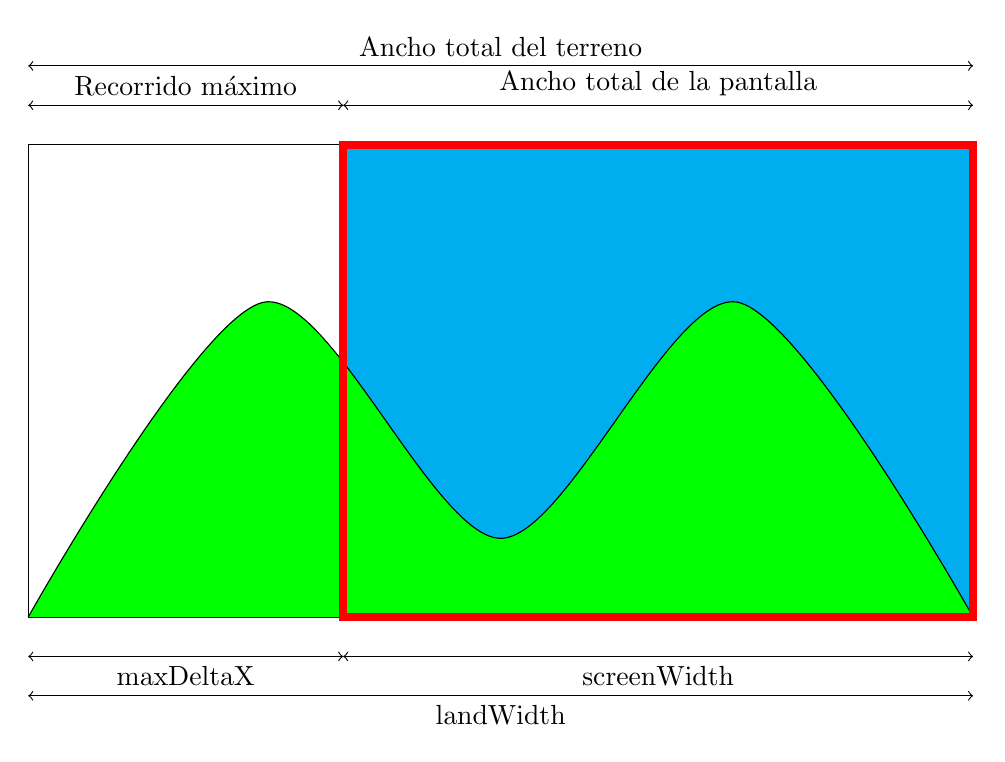
\begin{tikzpicture}
  \draw [<->] (0,7) -- node[above] {Ancho total del terreno} ++(12,0);
  \draw [<->] (0,6.5) -- node[above] {Recorrido máximo} ++(4,0) ;
  \draw [<->] (4,6.5) -- node[above] {Ancho total de la pantalla} ++(8,0);
  \draw (0,0) rectangle (12,6);
  \filldraw[fill=cyan, draw=black]  (4,0) rectangle (12,6);
  \fill[fill=green, draw=black] plot [smooth] coordinates {(0,0) (3,4) (6,1) (9,4) (12,0)};
  \draw [line width=1mm, red ] (4,0) rectangle (12,6);
  \draw [<->] (0,-0.5) -- node[below] {maxDeltaX} ++(4,0) ;
  \draw [<->] (4,-0.5) -- node[below] {screenWidth} ++(8,0);
  \draw [<->] (0,-1) -- node[below] {landWidth} ++(12,0);
\end{tikzpicture}

Estos valores pueden ser calculados y almacenados como propiedades del componente de la siguiente manera:

{\begin{lstlisting}[style=htmlcssjs,frame=tlrb, xleftmargin={0.2cm}]
export class HomePage implements AfterViewInit {
  /* Resto de variables */
  @ViewChild('landscape') landscapeElement:ElementRef; //nuestro div al que identificamos con el atributo #landscape
  maxDeltaX:number;
  currentDeltaX: number;
  lastPanDeltaX: number = 0;

  ngAfterViewInit() {
    var landWidth = this.landscapeElement.nativeElement.clientWidth;
    var screenWidth = this.landscapeElement.nativeElement.parentElement.clientWidth;
    this.maxDeltaX = (landWidth - screenWidth) * -1;
    this.currentDeltaX = this.maxDeltaX / 2; // Aprovechamos para centrar el terreno al iniciar.
  }
  /* Resto de funciones */
}
\end{lstlisting}}

\warningbox{Hay que tener en cuenta que el máximo desplazamiento se dará hacia la izquierda, por eso se trata de un número negativo. }

Con las medidas ya calculadas, vamos a tratar el gesto de desplazar el dedo sobre la pantalla. Ionic2 permite vincular los siguientes gestos desde el \emph{HTML}: \textbf{tap, press, pan, swipe, rotate y pinch}. Para nuestro propósito, el evento que necesitamos capturar es el de \textbf{pan} y lo haremos del mismo modo que capturamos el evento de click.

{\begin{lstlisting}[style=htmlcssjs,frame=tlrb, xleftmargin={0.2cm}]
<div class="canvas sky" [@skyState]="state" (pan)="panEvent(\$event)" >
  <div class="celestial sun" [@flyInOut] *ngIf="state === 'day'" (click)="toogleState()" ></div>
  <div class="celestial moon" [@flyInOut] *ngIf="state === 'night'" (click)="toogleState()" ></div>
  <div #landscape class="landscape" ></div>
</div>
\end{lstlisting}}

Veamos primero el código del método \emph{panEvent}, que es la que recoge y trata el gesto, y a continuación explicaré su funcionamiento.

{\begin{lstlisting}[style=htmlcssjs,frame=tlrb, xleftmargin={0.2cm}]
panEvent(e) {
  if (e.eventType == 4) {
    this.lastPanDeltaX = 0;
    return true;
  };
  var dx = e.deltaX - this.lastPanDeltaX;
  this.lastPanDeltaX = e.deltaX;

  if ((this.currentDeltaX + dx) < this.maxDeltaX || (this.currentDeltaX + dx) > 0) {
    return true;
  }
  this.currentDeltaX += dx;

  return true;
}
\end{lstlisting}}

Para entender este código hay que saber como funciona el evento que estamos capturando. Cada vez que se desplaza el dedo sobre la pantalla, por pocos píxeles que sean, se genera un evento que podemos capturar. Esto quiere decir que en caso de mover el dedo sin parar, el evento saltara cada pocos milisegundos. ¿Y que información nos proporciona?. Entre los múltiples parámetros\footnote{\url{https://hammerjs.github.io/api/\#event-object}} que tiene asociado el evento, el que nos indica el desplazamiento es \emph{deltaX} (también nos encontramos con los parámetros \emph{deltaY} y con \emph{distance}, pero en nuestro caso, solo nos interesa el movimiento horizontal). Este parámetro se mide en píxeles y representa la distancia recorrida horizontalmente desde el inicio del gesto. Como nos interesa actualizar la posición del terreno cada vez que se genera el evento para así conseguir que el dibujo se mueva al mismo tiempo que el dedo, necesitamos saber la distancia recorrida no al punto de inicio del gesto, si no al punto en el que se produjo el evento anterior. Para eso calculamos la diferencia entre la \emph{deltaX} del evento anterior, que guardamos en la variable \emph{lastPanDeltaX}, y la \emph{deltaX} del evento actual. Esta diferencia es la que se aplica al desplazamiento actual del terreno (\emph{currentDeltaX}) siempre y cuando entre dentro del desplazamiento permitido (de \emph{mapxDeltaX} a 0). ¿Y cuándo termina el gesto?. Cuando el usuario levanta el dedo, se lanza un último evento en el que el parámetro \emph{eventType}\footnote{\url{https://hammerjs.github.io/api/\#input-events}} toma el valor 4. En este momento, reseteamos \emph{lastPanDeltaX}.

Ahora que tenemos el desplazamiento que tenemos que aplicar a nuestro terreno, nos falta justamente eso, aplicárselo. Angular nos permite modificar el estilo de un elemento según una variable desde el HTML. Para realizar un desplazamiento lateral vamos a aplicar una transformación\footnote{\url{https://www.w3schools.com/cssref/css3_pr_transform.asp}} a nuestro elemento, mas concretamente, \emph{translateX()}, al cual se le pasa el desplazamiento medido en píxeles.

Normalmente para cambiar un estilo según el valor de una variable con Angular se haría lo siguiente:

{\begin{lstlisting}[style=htmlcssjs,frame=tlrb, xleftmargin={0.2cm}]
  <div [style.CSS_PROPERTY_NAME]=" VARIABLE " ></div>
\end{lstlisting}}

Pero en el caso del \emph{tranform}, esto viola algunas directivas de seguridad que aplica Angular, y es que sí, una de las cosas que Angular nos proporciona es protección contra las vulnerabilidades comunes que suelen tener las aplicaciones web \ldots aunque en esta ocasión interfiera con nuestros planes. Por suerte, existen mecanismos para saltarnos estas medidas de seguridad (bajo nuestra responsabilidad) para casos como el que nos ocupa. Estos mecanismos son conocidos como \emph{bypass}\footnote{\url{https://angular.io/docs/ts/latest/api/platform-browser/index/DomSanitizer-class.html}} y previenen de que el valor que les pasemos sea comprobado por los mecanismos de seguridad de Angular.

Para intentar dejar nuestro código lo más limpio posible, crearemos una tubería (ya vimos que son en la práctica del \nameref{sec:crono}) que al pasarle el valor numérico, nos genere el valor a asignar a la propiedad \emph{transform}.

{\begin{lstlisting}[style=htmlcssjs,frame=tlrb, xleftmargin={0.2cm}]
import { Pipe, PipeTransform } from '@angular/core';
import { DomSanitizer } from '@angular/platform-browser';

@Pipe({name: 'transform_sanitizer'})
export class TransformSanitizer implements PipeTransform {

  constructor(private sanitizer:DomSanitizer){}

  transform(deltaX) {
    return this.sanitizer.bypassSecurityTrustStyle("translateX(" + deltaX + "px)");
  }
}
\end{lstlisting}}

Ya solo nos quedaría añadirlo a nuestro \emph{HTML}:

{\begin{lstlisting}[style=htmlcssjs,frame=tlrb, xleftmargin={0.2cm}]
<div class="canvas sky" [@skyState]="state" (pan)="panEvent(\$event)" >
  <div class="celestial sun" [@flyInOut] *ngIf="state === 'day'" (click)="toogleState()" ></div>
  <div class="celestial moon" [@flyInOut] *ngIf="state === 'night'" (click)="toogleState()" ></div>
  <div #landscape [style.transform]="currentDeltaX | transform_sanitizer" class="landscape" ></div>
</div>
\end{lstlisting}}

\subsection{Animación CSS. El ave.}

Nuestro siguiente paso será incluir un habitante en nuestro paisaje, yo me he decantado por un pájaro. Nuestro nuevo amigo estará de pie sobre el terreno, por ello, es necesario que se mueva cuando desplacemos todo el terreno. Para conseguirlo, el elemento que representa a este pájaro dentro del \emph{div} del terreno. Veamos el código:

\noindent
\begin{minipage}[t]{.48\textwidth}
{\begin{lstlisting}[style=htmlcssjs,frame=tlrb, xleftmargin={0.2cm}]
<div class="canvas sky" [@skyState]="state" (pan)="panEvent(\$event)" >
  <div class="celestial sun" [@flyInOut] *ngIf="state === 'day'" (click)="toogleState()" ></div>
  <div class="celestial moon" [@flyInOut] *ngIf="state === 'night'" (click)="toogleState()" ></div>
  <div #landscape [style.transform]="currentDeltaX | transform_sanitizer" class="landscape" >
    <div class="bird" [@birdState]="state" ></div>
  </div>
</div>
\end{lstlisting}}
\end{minipage}\hfill
\noindent
\begin{minipage}[t]{.48\textwidth}
{\begin{lstlisting}[style=htmlcssjs,frame=tlrb, xleftmargin={0.2cm}]
page-home {
  .canvas.sky{ ... }
  .celestial{ ... }
  .landscape {
    // Resto de propiedades.
    .bird {
      position: fixed;
      height: 100px;
      width: 100px;
      left: 30%;
      top: 60%;
      background-size: 100% 100%;
      background-repeat: no-repeat;
      pointer-events: none;
    }
  }
}
\end{lstlisting}}
\end{minipage}

Ya que la fauna diurna no es la misma que la que nos encontramos en la noche, vamos a cambiar la especie de nuestro habitante utilizando una animación que modifique la imagen que se utiliza:

{\begin{lstlisting}[style=htmlcssjs,frame=tlrb, xleftmargin={0.2cm}]
trigger('birdState', [
  state('day', style({
    'background-image': 'url(../assets/landscape/bird.png)'
  })),
  state('night',   style({
    'background-image': 'url(../assets/landscape/owl.png)'
  })),
  transition('day <=> night', animate('0.5s 0.5s')), // La animación dura 0.5 segundos y empiza 0.5 segundos retrasada
]),
\end{lstlisting}}

Para animar un poco a nuestro pájaro, y no parezca que se trata de una objeto sin vida, vamos a añadirle un poco de movimiento, y como no, vamos a usar una animación para esto. En este caso, al tratarse de una animación que se repite en el tiempo y de la que conocemos tanto su estado inicial como final e intermedios, definiremos la animación directamente en el \gls{CSS}. Vamos a definir dos animaciones diferentes, durante el día, nuestro pájaro pivoteará de un lado a otro, y durante la noche, pegará saltos. \gls{CSS} nos permite definir \emph{keyframes}, en los que indicar el estilo según el porcentaje de animación que se haya completado.

{\begin{lstlisting}[style=htmlcssjs,frame=tlrb, xleftmargin={0.2cm}]
@keyframes spin {
    0%, 45%   {transform: rotateY(0deg);} // En el 45% empezará a cambiar
    50%, 95%  {transform: rotateY(180deg);} // En el 50% ya se habrá realizado el cambio
}

@keyframes jump {
    0%, 45%, 55%   {top: 60%}
    50%  {top: 50%} // Al punto más alto se llega a mitad de la animación
}
\end{lstlisting}}

Completamos el estilo de nuestro elemento para añadir la animación. En este caso le pondremos por defecto la animación \emph{spin} (y así ver en conjunto todas las opciones de la animación), aunque como veremos a continuación, esta animación cambiará junto al estado.

{\begin{lstlisting}[style=htmlcssjs,frame=tlrb, xleftmargin={0.2cm}]
.bird {
  position: fixed;
  height: 100px;
  width: 100px;
  left: 30%;
  top: 60%;
  background-size: 100% 100%;
  background-repeat: no-repeat;
  pointer-events: none;
  animation-name: spin;
  animation-duration: 6s;
  animation-iteration-count: infinite;
  animation-timing-function: easeInQuint // https://www.w3schools.com/cssref/css3_pr_animation-timing-function.asp;
}
\end{lstlisting}}

En nuestro componente cambiamos la definición del trigger \emph{birdState}:

{\begin{lstlisting}[style=htmlcssjs,frame=tlrb, xleftmargin={0.2cm}]
trigger('birdState', [
  state('day', style({
    'background-image': 'url(../assets/landscape/bird.png)',
    'animation-name': 'spin',
    'animation-duration': '6s'
  })),
  state('night',   style({
    'background-image': 'url(../assets/landscape/owl.png)',
    'animation-name': 'jump',
    'animation-duration': '3s'
  })),
  transition('day <=> night', animate('0.5s 0.5s')),
])
\end{lstlisting}}

Veamos como funciona la animación de giro con la configuración especificada. En primer lugar, la animación durará 6s. Esto, junto con la definición del \emph{keyframe} tenemos que:

\begin{enumerate}
  \item El elemento empieza rotado 0 grados.
  \item En el segundo 6*0.45 = 2.7, empieza la animación de giro.
  \item En el segundo 6*0.5 = 3, el elemento está rotado 180 grados.
  \item En el segundo 6*0.95 = 5.7, el elemento empieza a rotar hacia la posición original.
  \item En el segundo 6*1 = 6, el elemento está en la posición original.
  \item Vuelta a empezar.
\end{enumerate}

El funcionamento es análoco en la definición del salto.

\subsection{Elementos extras. Sonidos y nubes.}


Como broche final a nuestro paisaje, vamos a hacer que se reproduzca un sonido, en nuestro caso el canto del pájaro, cuando se realiza el cambio de estado. Las animaciones de Angular permiten asignar desde el \emph{HTML} una acción tanto al comienzo de la animación, como al finalizarla.

{\begin{lstlisting}[style=htmlcssjs,frame=tlrb, xleftmargin={0.2cm}]
<div #landscape [style.transform]="currentDeltaX | transform_sanitizer" class="landscape" >
  <div #bird class="bird" (@birdState.start)="playAudio() " [@birdState]="state" ></div>
</div>
\end{lstlisting}}

{\begin{lstlisting}[style=htmlcssjs,frame=tlrb, xleftmargin={0.2cm}]
export class HomePage implements AfterViewInit {
  //Resto de variables
  audio: any;

  //Resto de funciones
  playAudio() {
    if (this.audio) { //Nos aseguramos de que si existe algún sonido reproduciéndose, lo detenemos
      this.audio.pause();
    }
    this.audio = 'day' == this.state ? new Audio('../assets/sounds/bird.mp3') : new Audio('../assets/sounds/owl.mp3');
    this.audio.play();
  }
}
\end{lstlisting}}

Con esto ya tendríamos completo nuestro paisaje. Podemos añadir más elementos si queremos poner en práctica lo aprendido o probar cosas nuevas, por ejemplo, yo he añadido unas nubes que también se mueven junto con el terreno, pero a una velocidad menor.

\noindent
\begin{minipage}[t]{.48\textwidth}
{\begin{lstlisting}[style=htmlcssjs,frame=tlrb, xleftmargin={0.2cm}]
<div class="canvas sky" [@skyState]="state" (pan)="panEvent(\$event)" >
  <div class="celestial sun" [@flyInOut] *ngIf="state === 'day'" (click)="toogleState()" ></div>
  <div class="celestial moon" [@flyInOut] *ngIf="state === 'night'" (click)="toogleState()" ></div>
  <div [style.transform]="currentDeltaX / 3 | transform_sanitizer" class="cloud left" ></div>
  <div [style.transform]="currentDeltaX / 3 | transform_sanitizer" class="cloud rigth" ></div>
  <div #landscape [style.transform]="currentDeltaX | transform_sanitizer" class="landscape" >
    <div class="bird" (@birdState.start)="playAudio()" [@birdState]="state" ></div>
  </div>
</div>

\end{lstlisting}}
\end{minipage}\hfill
\noindent
\begin{minipage}[t]{.48\textwidth}
{\begin{lstlisting}[style=htmlcssjs,frame=tlrb, xleftmargin={0.2cm}]
page-home {
  .canvas.sky{ ...
    .celestial{ ... }
    .cloud {
      position: fixed;
      height: 60px;
      width: 150px;
      background-image: url(../assets/landscape/cloud.png);
      background-size: 100% 100%;
      background-repeat: no-repeat;
      pointer-events: none;
      &.left {
        top: 8%;
        left: 25%;
      }
      &.rigth {
        top: 12%;
        left: 65%;
      }
    }
    .landscape { ... }
  }
}
\end{lstlisting}}
\end{minipage}

\subsection{Apunte final y uso de animaciones en otros escenarios.}

Con esta práctica he querido abarcar diferentes formas de crear animaciones cuando se trata de una aplicación hecha con Ionic2. Se puede conseguir el mismo resultado aplicando métodos distintos. Por ejemplo, haciendo las animaciones solo con JS, utilizar jQuery u alguna otra librería externa, \ldots.

Como último apunte, indicar que aunque en este caso hemos estado animando elementos que representaban imágenes para intentar hacer la explicación más visual y llamativa, no debemos pensar que las animaciones solo se utilizan para hacer "dibujitos". Las animaciones se pueden aplicar a cualquier elemento del árbol \gls{DOM} y a cualquier regla que se pueda definir en \gls{CSS}. Un ejemplo muy utilizado sería cambiar el tamaño de fuente en un texto cuándo nos posicionamos sobre él:

{\begin{lstlisting}[style=htmlcssjs,frame=tlrb, xleftmargin={0.2cm}]
<head>
  <style media="screen" >
    .text {
      font-size: 14px;
      transition: font-size 1s ease-in; \\ Manera abreviada de definir una transición
    }
    .text:hover {
      font-size: 40px;
    }
  </style>
</head>
<body>
  <div class="text" >
    Pasa sobre mí el ratón.
  </div>
</body>
\end{lstlisting}}

O desplegar un menú lateral:

{\begin{lstlisting}[style=htmlcssjs,frame=tlrb, xleftmargin={0.2cm}]
<head>
  <style media="screen" >
    body {
      display: flex;
      height: 100%;
    }
    div {
      height: 100%;
    }
    div.menu {
      background-color: green;
      width: 20px;
      transition: width 1s, background-color 1s;
    }
    div.menu:hover {
      background-color: yellow;
      width: 200px;
    }
    div.main {
      background-color: cyan;
      flex-grow: 1;
    }
    button {
      min-width: 200px
    }
  </style>
</head>
<body>
  <div class="menu" >
    <button>OPTION 1</button>
    <button>OPTION 2</button>
    <button>OPTION 3</button>
  </div>
  <div class="main" ></div>
</body>
\end{lstlisting}}
